% Created 2025-03-10 Mon 01:56
% Intended LaTeX compiler: lualatex
\documentclass[bigger]{beamer}
\usepackage{amsmath}
\usepackage{fontspec}
\usepackage{graphicx}
\usepackage{longtable}
\usepackage{wrapfig}
\usepackage{rotating}
\usepackage[normalem]{ulem}
\usepackage{capt-of}
\usepackage{hyperref}
\usetheme[progressbar=foot, sectionpage=none, numbering=fraction]{metropolis}
\usepackage{tikz}
\usepackage{booktabs}
\usepackage{adjustbox}
\usepackage{diagbox}
\usepackage{latexcolors}
\usetikzlibrary{automata, positioning, arrows, arrows.meta}
\usepackage{diagbox}
\usepackage{dsfont}
\usepackage{amsmath}
\usepackage{fontawesome}
\usepackage{pgfgantt}
\usepackage[ruled]{algorithm2e}
\usepackage[absolute, overlay]{textpos}
\usepackage{xcolor}
\definecolor{UmlBlue}{HTML}{0067b1} \setbeamercolor{progress bar}{fg=UmlBlue} \setbeamercolor{title separator}{fg=UmlBlue}
\setbeamercolor{progress bar in head/foot}{fg=UmlBlue} \setbeamercolor{progress bar in section page}{fg=UmlBlue} \setbeamercolor{alerted text}{fg=UmlBlue}
\pretocmd{\tableofcontents}{\thispagestyle{empty}}{}{}
\usetheme{default}
\author{Andrea Pierré}
\date{March 11, 2025}
\title{Lab meeting}
\subtitle{\emph{Robust representations for olfactory-spatial association learning}}
\setbeamercovered{transparent=10}
\setbeamertemplate{section in toc}[sections numbered]
\AtBeginSection[]{\begin{frame}[plain, noframenumbering]{Outline}    \setbeamertemplate{section in toc}[sections numbered]\setbeamertemplate{subsection in toc}[subsections numbered]\tableofcontents[currentsection, currentsubsection]\end{frame}}
\AtBeginSubsection[]{\begin{frame}[plain, noframenumbering]{Outline}\setbeamertemplate{section in toc}[sections numbered]\setbeamertemplate{subsection in toc}[subsections numbered]\tableofcontents[currentsection,currentsubsection]\end{frame}}
\definecolor{headercolor}{HTML}{232323}
\setbeamercolor{normal text}{%
% bg=,
fg=headercolor
}
\hypersetup{
 pdfauthor={Andrea Pierré},
 pdftitle={Lab meeting},
 pdfkeywords={},
 pdfsubject={},
 pdfcreator={Emacs 29.4 (Org mode 9.7.19)}, 
 pdflang={English}}
\begin{document}

\maketitle
\begin{frame}[plain]{Outline}
\tableofcontents
\end{frame}

\section{Project recap}
\label{sec:org8c7a89d}
\begin{frame}[label={sec:org05abde2}]{The LEC is key to sensory associations and spatial memory}
\begin{columns}
\begin{column}{0.45\columnwidth}
\footnotesize
\begin{itemize}
\item \alert{Piriform Cortex} encodes olfactory information
\item \alert{Hippocampus} encodes spatial information
\item \alert{Lateral Entorhinal Cortex (LEC)} encodes both olfactory \& spatial information
\end{itemize}
\end{column}
\begin{column}{0.55\columnwidth}
\begin{center}
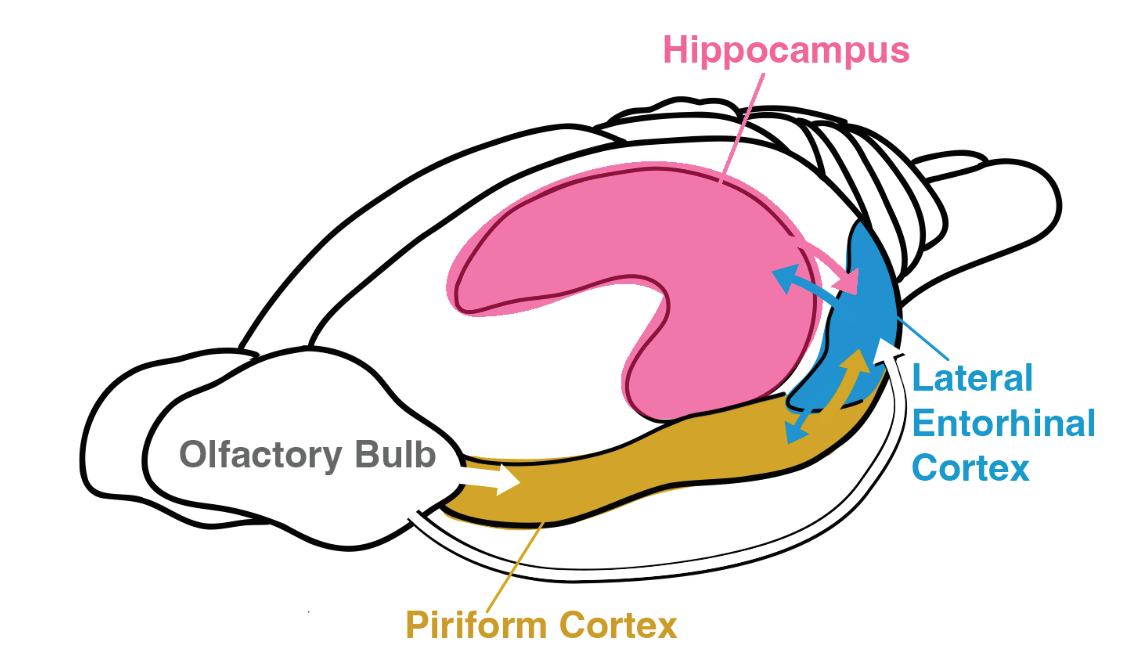
\includegraphics[width=\textwidth]{img/brain.png}
\end{center}

\begin{textblock}{5}(0.5,14.5)%
\tiny
Poo et al., 2022\\
Bitzenhofer et al., 2022\\
Lee et al., 2021
\end{textblock}
\end{column}
\end{columns}
\end{frame}
\begin{frame}[label={sec:org2840a5c}]{Half triangle task for olfactory-spatial association learning}
\begin{columns}
\begin{column}[c]{0.33\columnwidth}
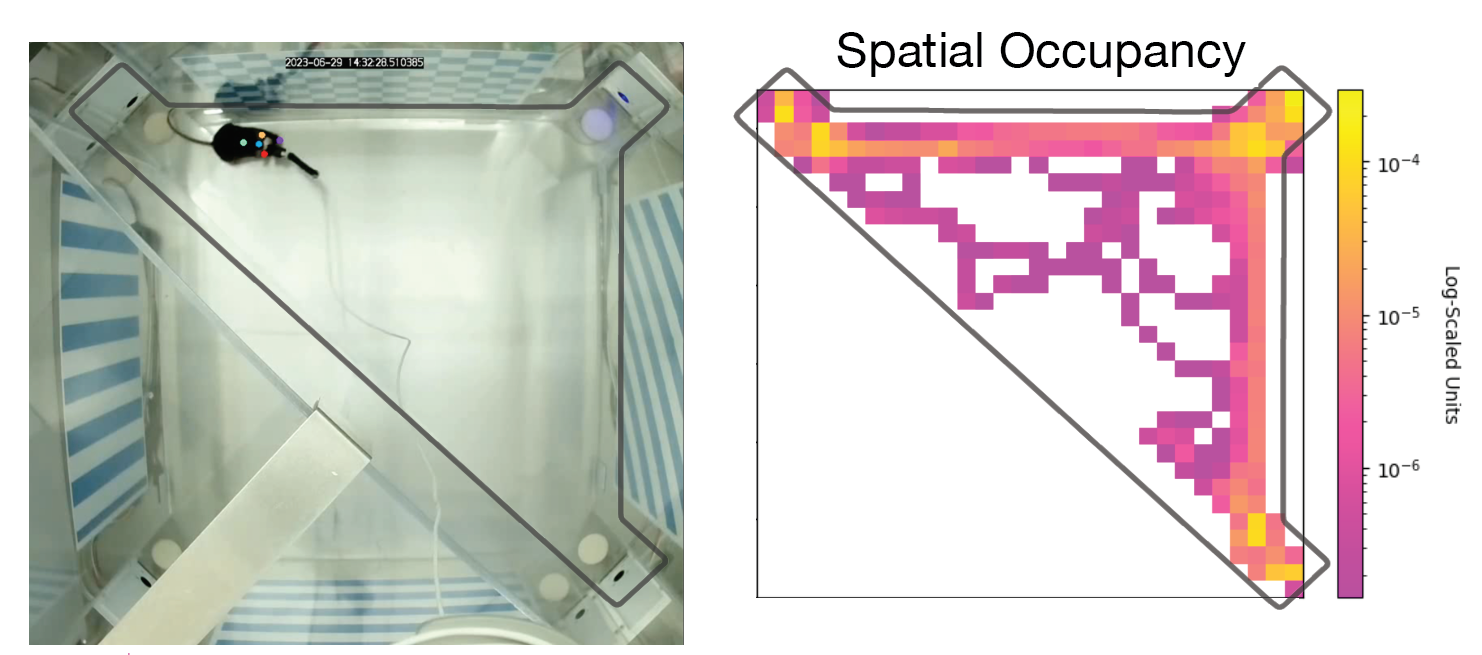
\includegraphics[width=\linewidth, keepaspectratio, trim={0cm 0cm 28cm 0cm}, clip]{img/video-picture.png}
\end{column}
\begin{column}[c]{0.33\columnwidth}
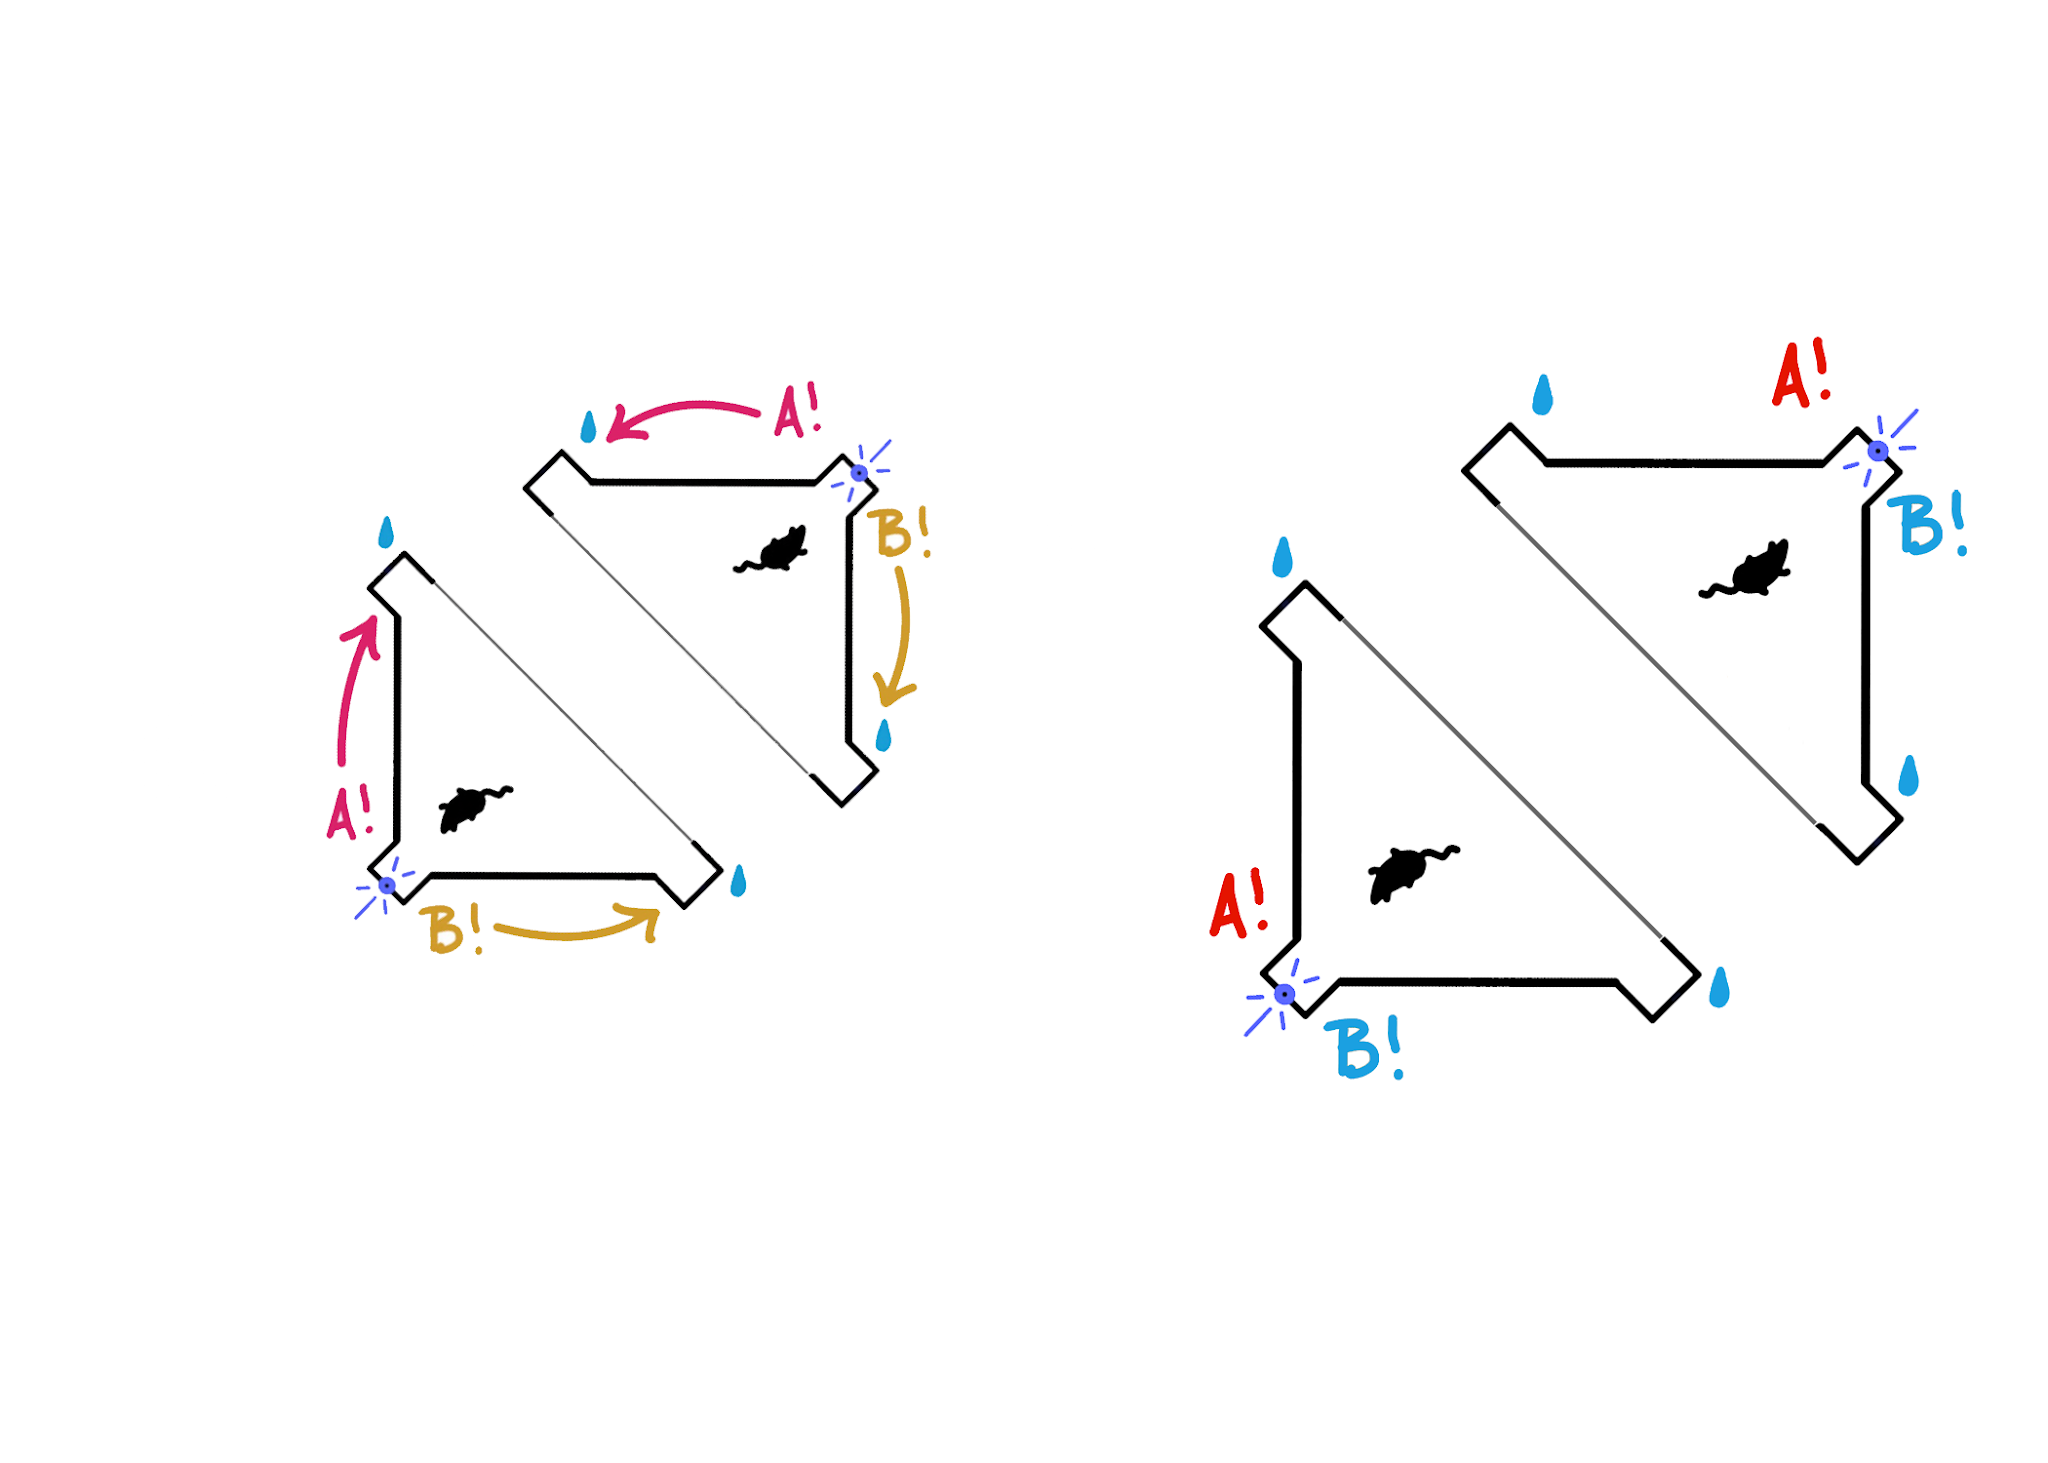
\includegraphics[width=0.9\linewidth, keepaspectratio, trim={11cm 18cm 40cm 13cm}, clip]{img/task-east-west.png}
\end{column}
\begin{column}[c]{0.33\columnwidth}
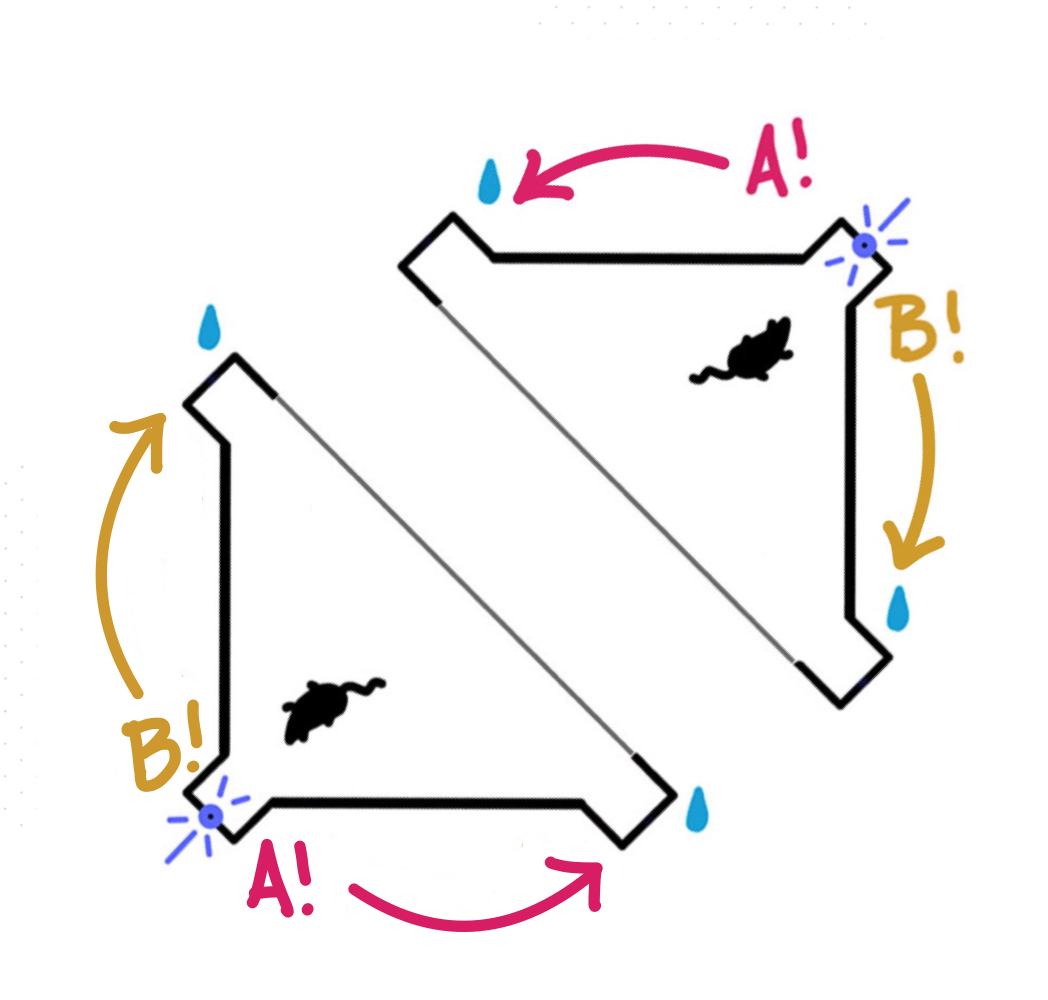
\includegraphics[width=0.9\linewidth, keepaspectratio, trim={3cm 2cm 4cm 4cm}, clip]{img/task-left-right.jpeg}
\end{column}
\end{columns}
\end{frame}
\begin{frame}[label={sec:org1e376a0}]{Deep Reinforcement Learning model}
\begin{center}
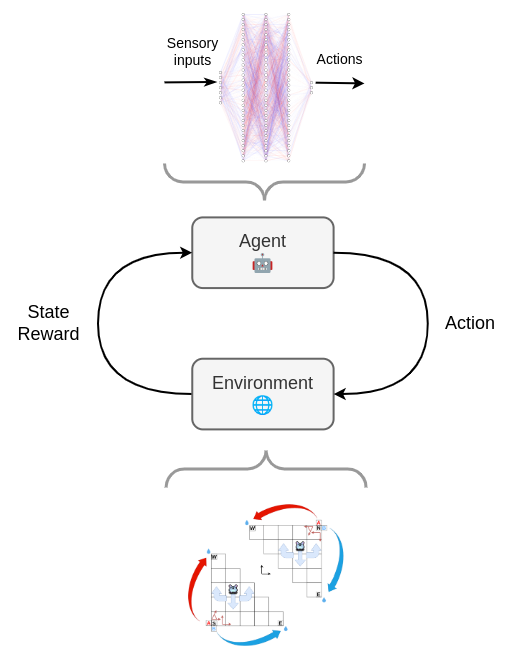
\includegraphics[height=0.95\textheight]{img/nn.drawio.png}
\end{center}
\end{frame}
\begin{frame}[label={sec:orgae968a5}]{Cartesian/polar duplicated coordinates experiment}
\begin{center}
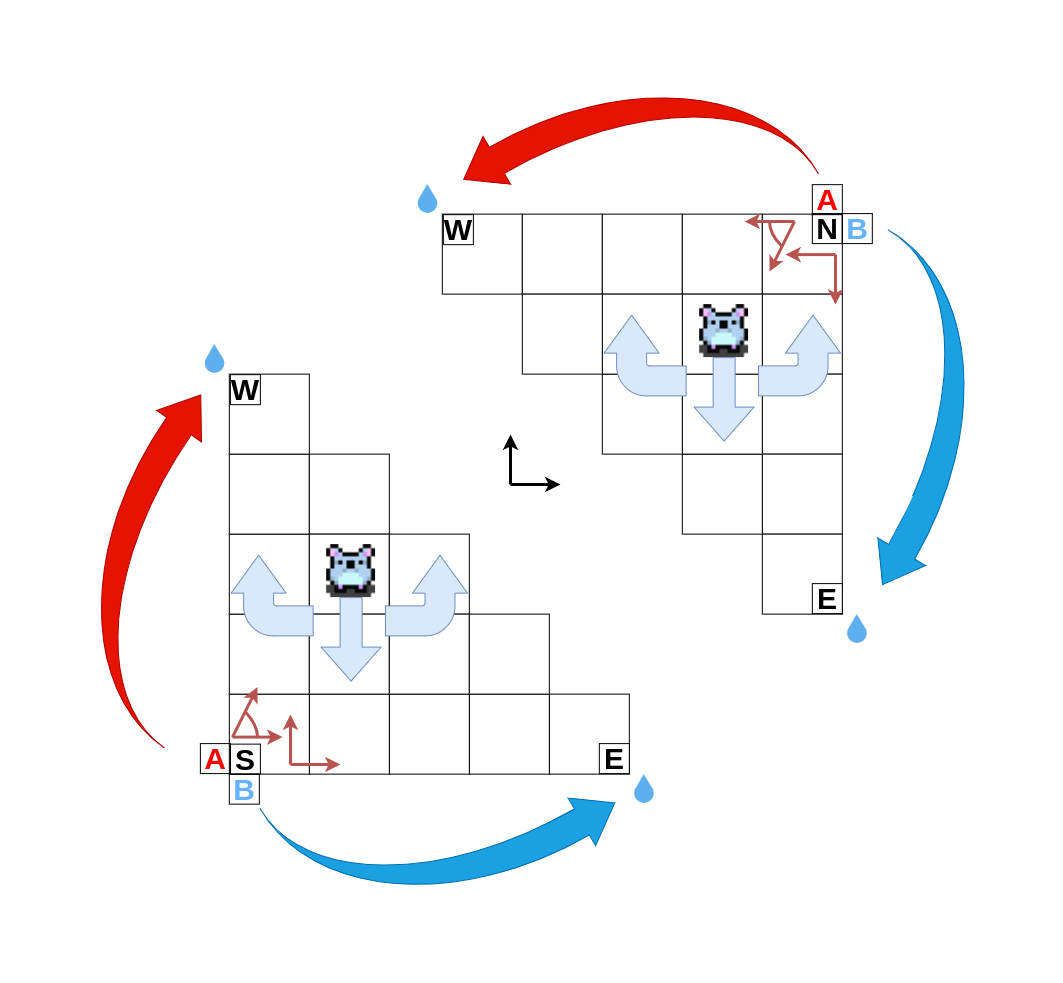
\includegraphics[height=0.6\textheight]{img/RL_env-cartesian-polar.drawio.png}
\end{center}
\footnotesize
\vspace{-1em}
\begin{itemize}
\item 3 actions: \(\Leftarrow \quad \Uparrow \quad \Rightarrow\)
\item Duplicated coordinates inputs:
\begin{itemize}
\item Cartesian coordinates from north \& south port
\item Polar coordinates from north \& south port
\end{itemize}
\end{itemize}
\end{frame}
\begin{frame}[label={sec:org8d59d68}]{Questions \& Hypothesis}
\metroset{block=fill}
\begin{exampleblock}{Questions}
\begin{itemize}
\item What \alert{function} does the network learn?
\item How the constrains of the task affect learning \& the representations learned?
%\item How this task structure might employ different representations of the action space?
\item How do the representations learned compare between the \emph{in vivo} and the \emph{in silico} neurons?
\end{itemize}
\end{exampleblock}
\pause
\begin{exampleblock}{Hypothesis}
\begin{itemize}
\item The network will use the most efficient coordinate information based on the task
\item The structure of the network's weights will reflect this prioritization of information
\end{itemize}
\end{exampleblock}
\end{frame}
\begin{frame}[label={sec:org07ba994}]{Looking back\(\dots\)}
\footnotesize
\begin{center}
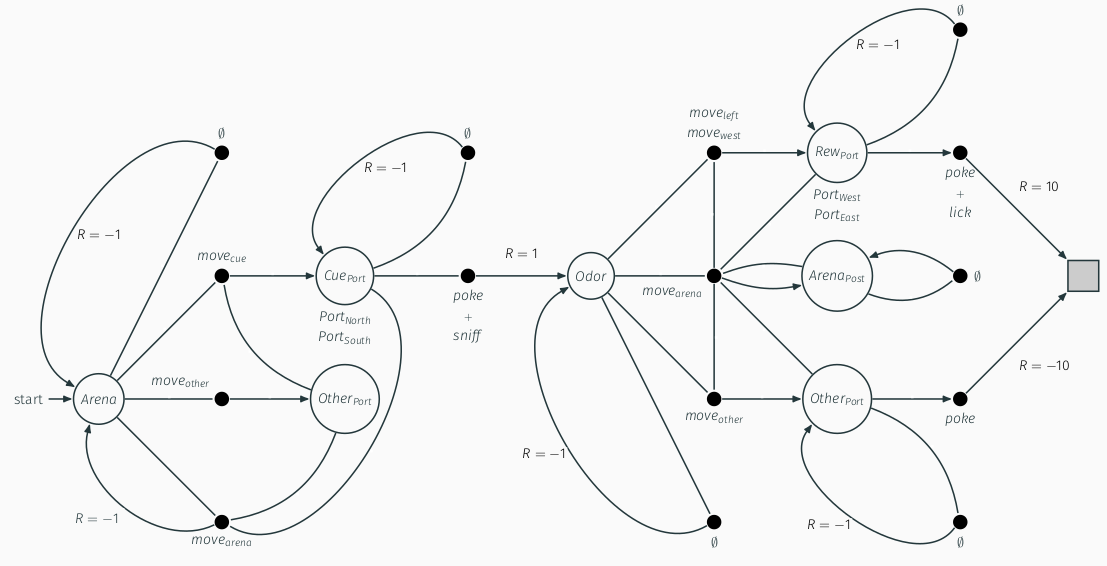
\includegraphics[height=0.5\textheight]{img/mdp.png}
\end{center}
\begin{enumerate}
\item Try to define the Olivia's experiment as a Markov Decision Process (MDP) in Julia
\item 2D gridworld in Python/NumPy
\item Duplicated coordinates in Python/PyTorch
\end{enumerate}
\end{frame}
\section{Cartesian/polar duplicated coordinates experiment}
\label{sec:org1c6e01f}
\begin{frame}[label={sec:org7bb1314}]{State space \& network architecture}
\begin{center}
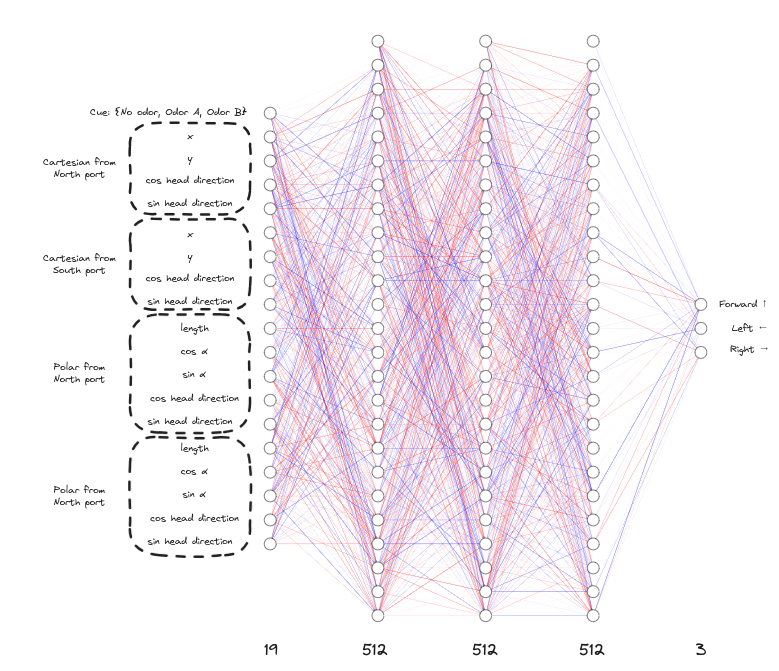
\includegraphics[height=0.95\textheight]{img/state-space-nn.png}
\end{center}
\end{frame}
\begin{frame}[label={sec:org93ab9d8}]{Training}
East/West
\begin{center}
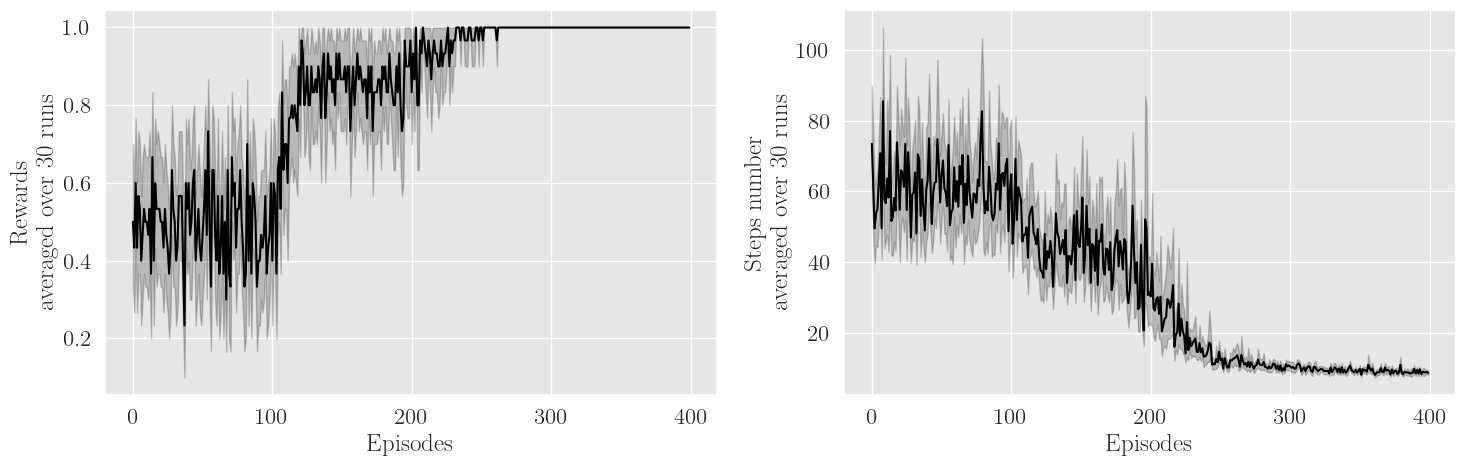
\includegraphics[height=0.35\textheight]{img/steps-and-rewards-EastWest.png}
\end{center}
Left/Right
\begin{center}
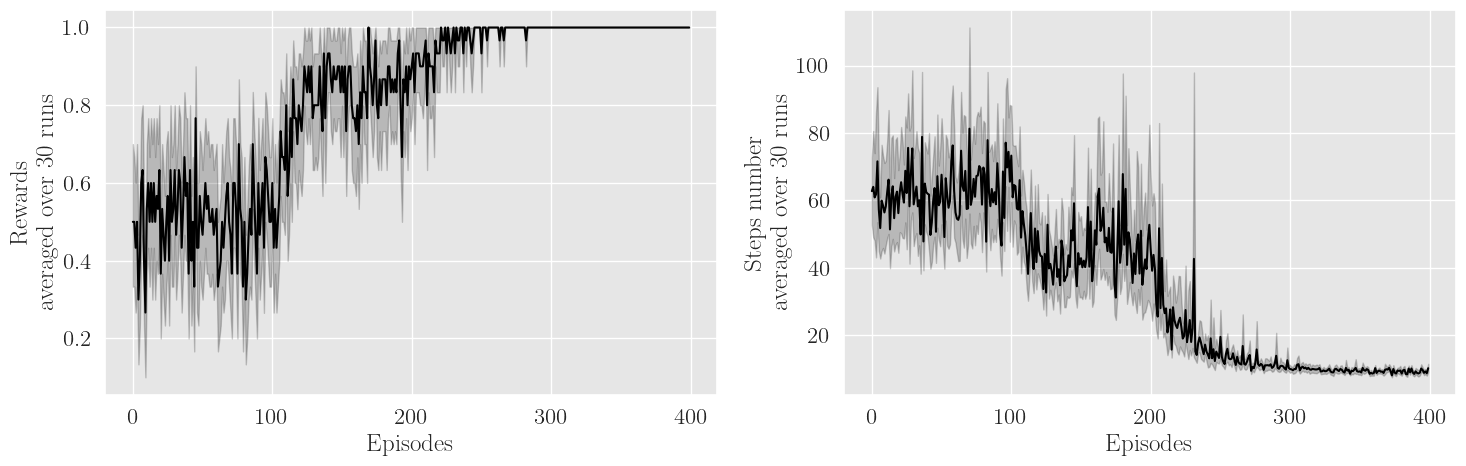
\includegraphics[height=0.35\textheight]{img/steps-and-rewards-LeftRight.png}
\end{center}
\end{frame}
\begin{frame}[label={sec:orgf839386}]{Training checks - East/West}
\begin{center}
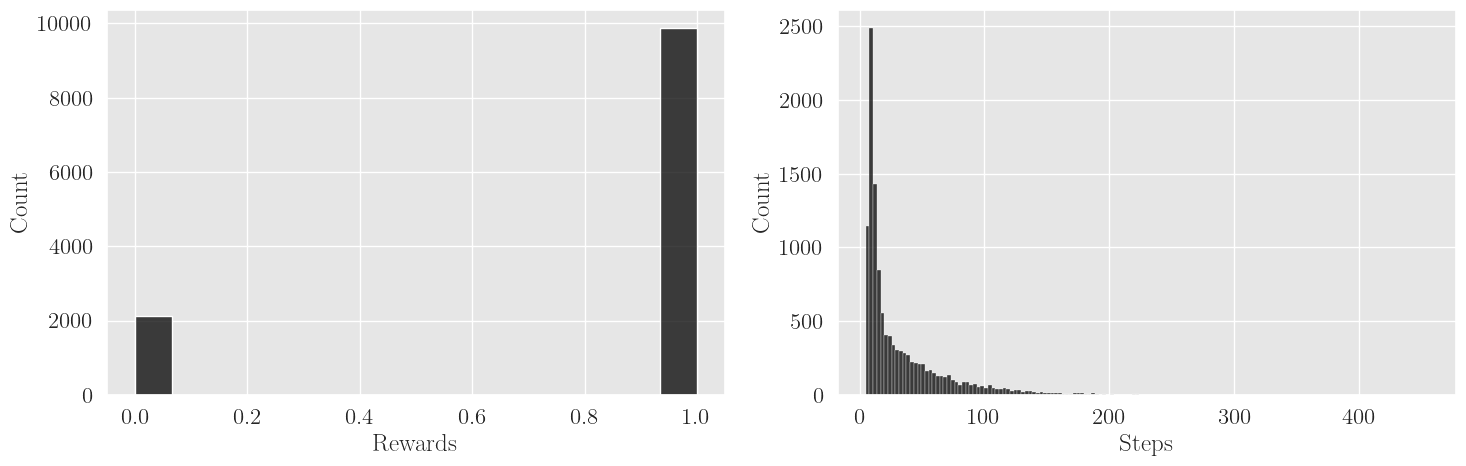
\includegraphics[width=\textwidth]{img/steps-and-rewards-distrib-EastWest.png}
\end{center}
\begin{columns}
\begin{column}[c]{0.5\columnwidth}
\begin{center}
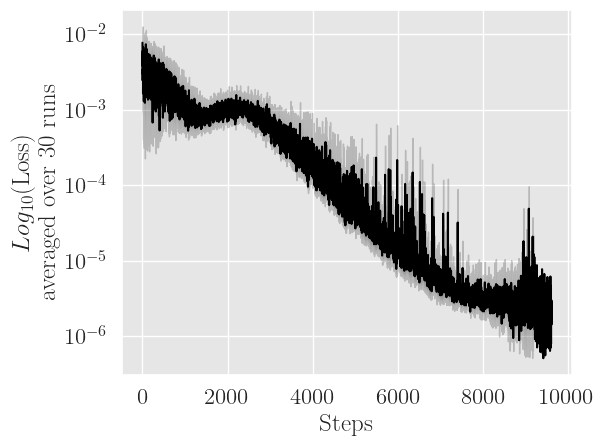
\includegraphics[width=0.8\textwidth]{img/loss-EastWest.png}
\end{center}
\end{column}
\begin{column}[c]{0.5\columnwidth}
\begin{center}
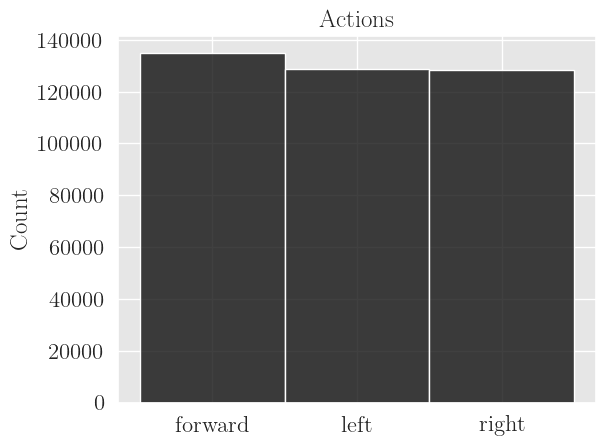
\includegraphics[width=0.65\textwidth]{img/actions-distribution-EastWest.png}
\end{center}
\end{column}
\end{columns}
\end{frame}
\begin{frame}[label={sec:org8c5ae25}]{Training checks - Left/Right}
\begin{center}
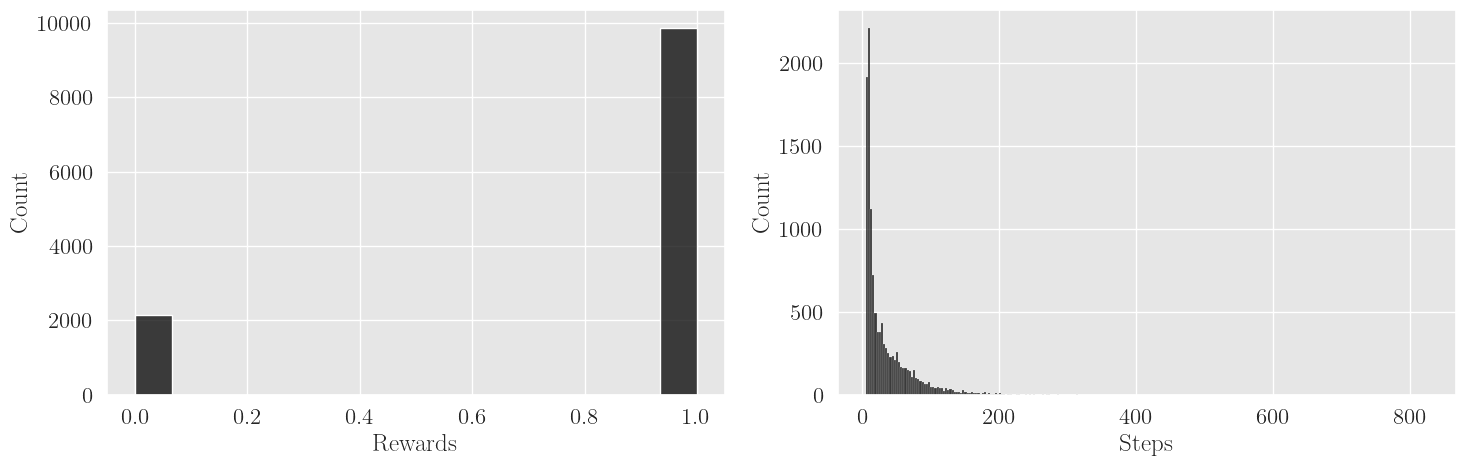
\includegraphics[width=\textwidth]{img/steps-and-rewards-distrib-LeftRight.png}
\end{center}
\begin{columns}
\begin{column}[c]{0.5\columnwidth}
\begin{center}
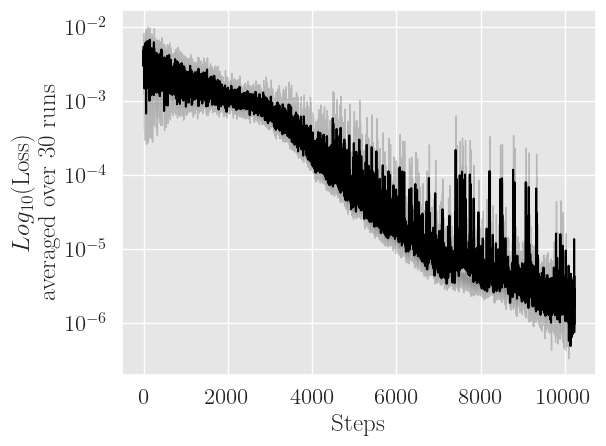
\includegraphics[width=0.8\textwidth]{img/loss-LeftRight.png}
\end{center}
\end{column}
\begin{column}[c]{0.5\columnwidth}
\begin{center}
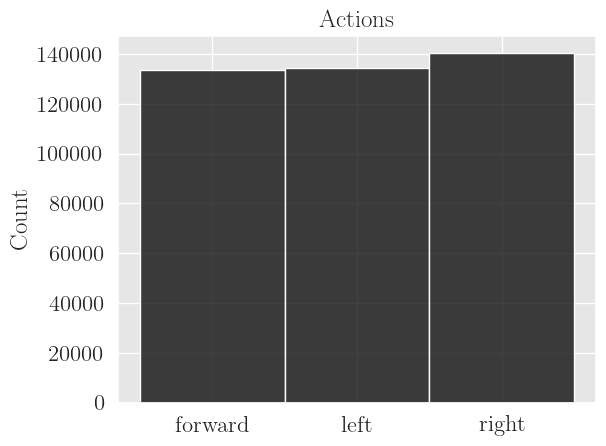
\includegraphics[width=0.65\textwidth]{img/actions-distribution-LeftRight.png}
\end{center}
\end{column}
\end{columns}
\end{frame}
\begin{frame}[label={sec:org9499775}]{Agent behavior}
\begin{columns}
\begin{column}[c]{0.3\columnwidth}
\begin{center}
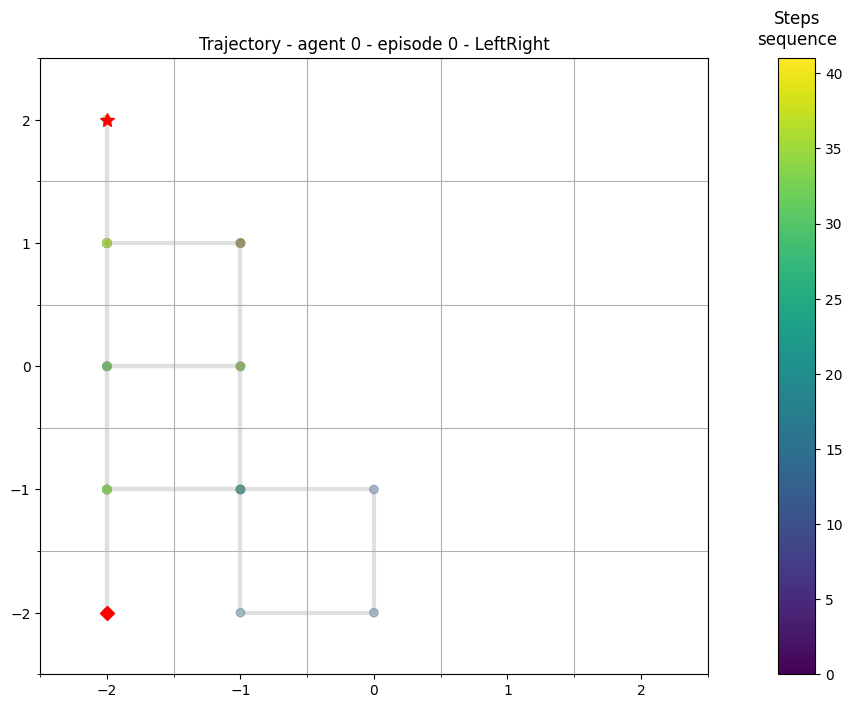
\includegraphics[height=0.28\textheight]{img/trajectory-0-0-LeftRight.png}
\end{center}
\begin{center}
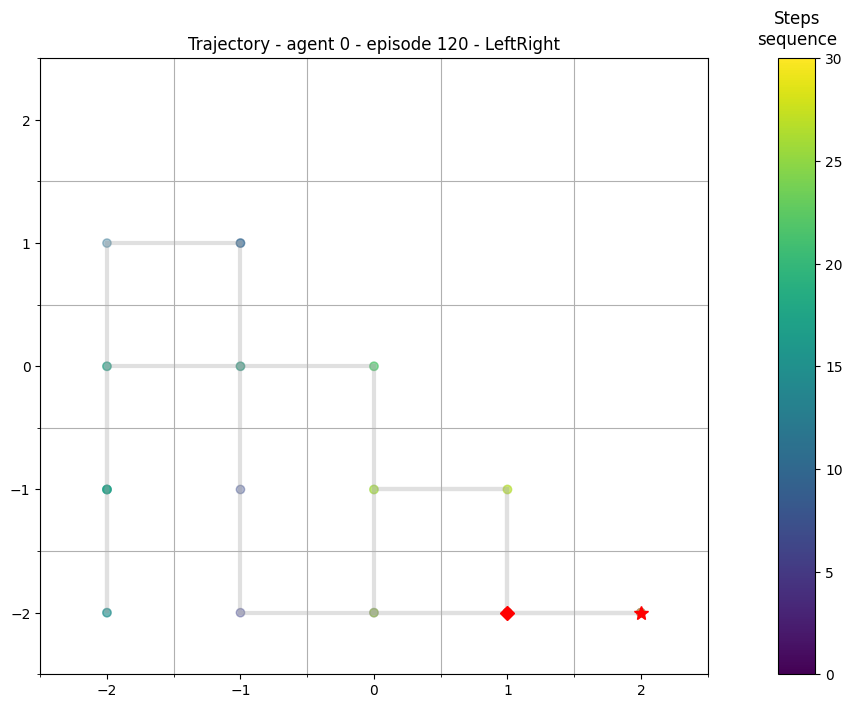
\includegraphics[height=0.28\textheight]{img/trajectory-0-120-LeftRight.png}
\end{center}
\begin{center}
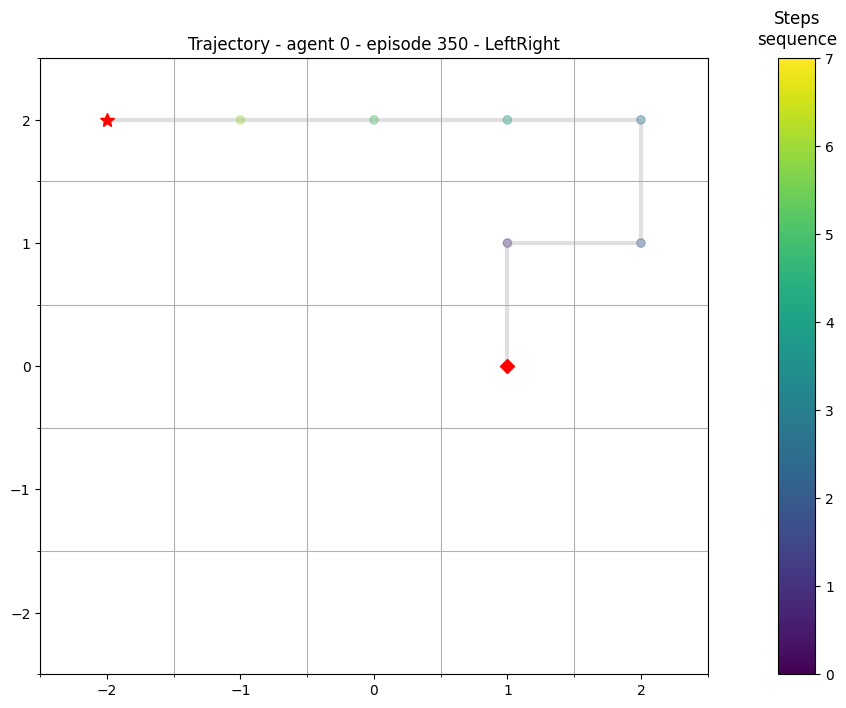
\includegraphics[height=0.28\textheight]{img/trajectory-0-350-LeftRight.png}
\end{center}
\end{column}
\begin{column}[c]{0.3\columnwidth}
\begin{center}
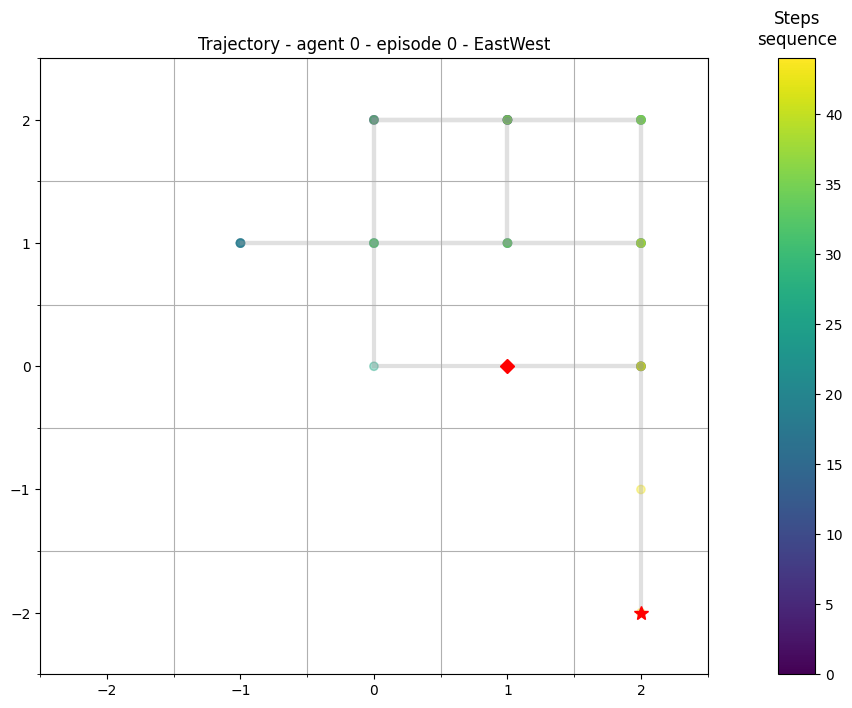
\includegraphics[height=0.28\textheight]{img/trajectory-0-0-EastWest.png}
\end{center}
\begin{center}
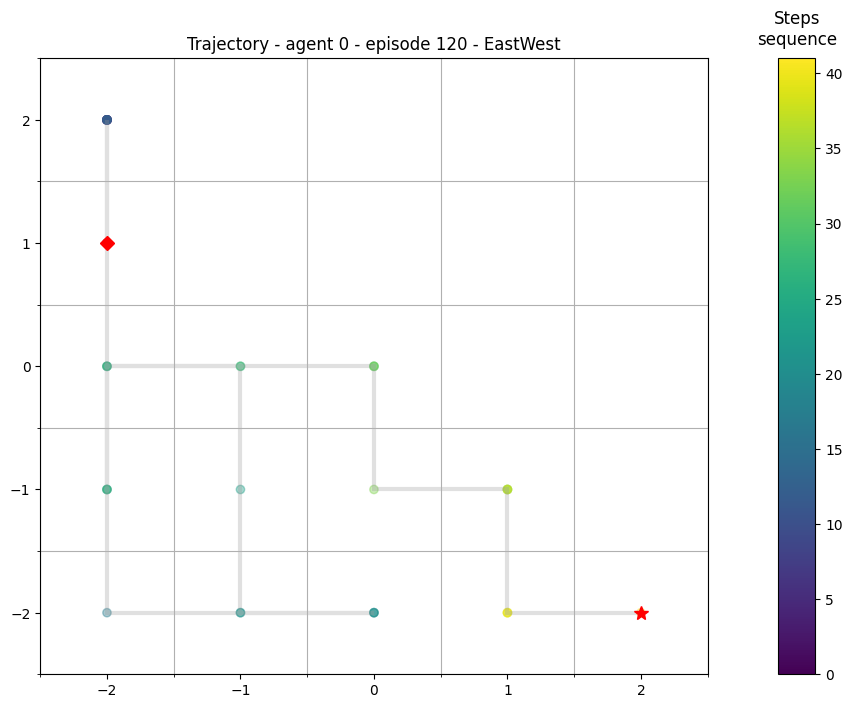
\includegraphics[height=0.28\textheight]{img/trajectory-0-120-EastWest.png}
\end{center}
\begin{center}
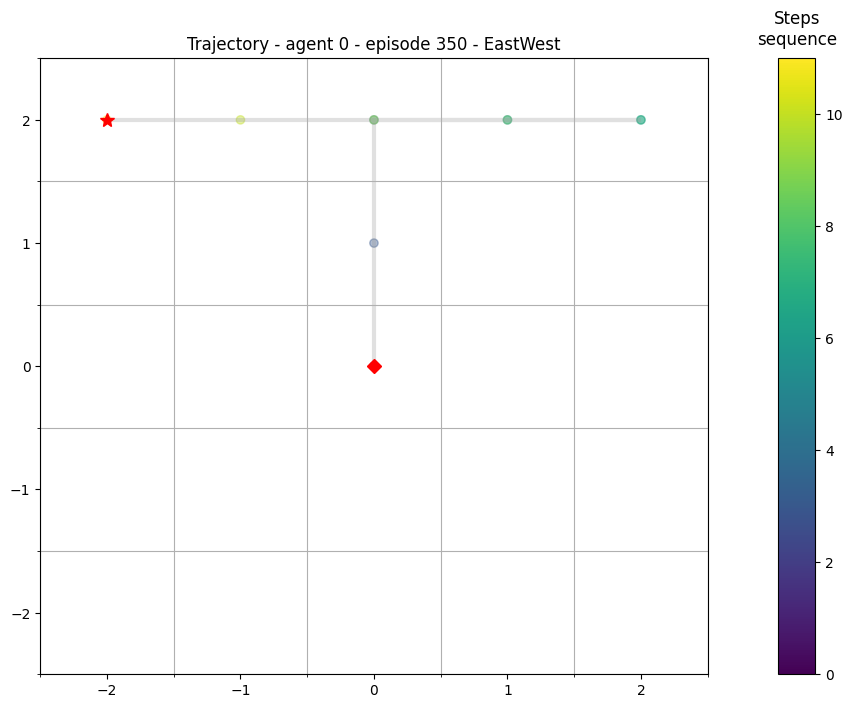
\includegraphics[height=0.28\textheight]{img/trajectory-0-350-EastWest.png}
\end{center}
\end{column}
\end{columns}
\end{frame}
\section{What does the network learn?}
\label{sec:org5fb47e4}
\begin{frame}[label={sec:orgf9298d6}]{Activations learned - East/West}
\begin{center}
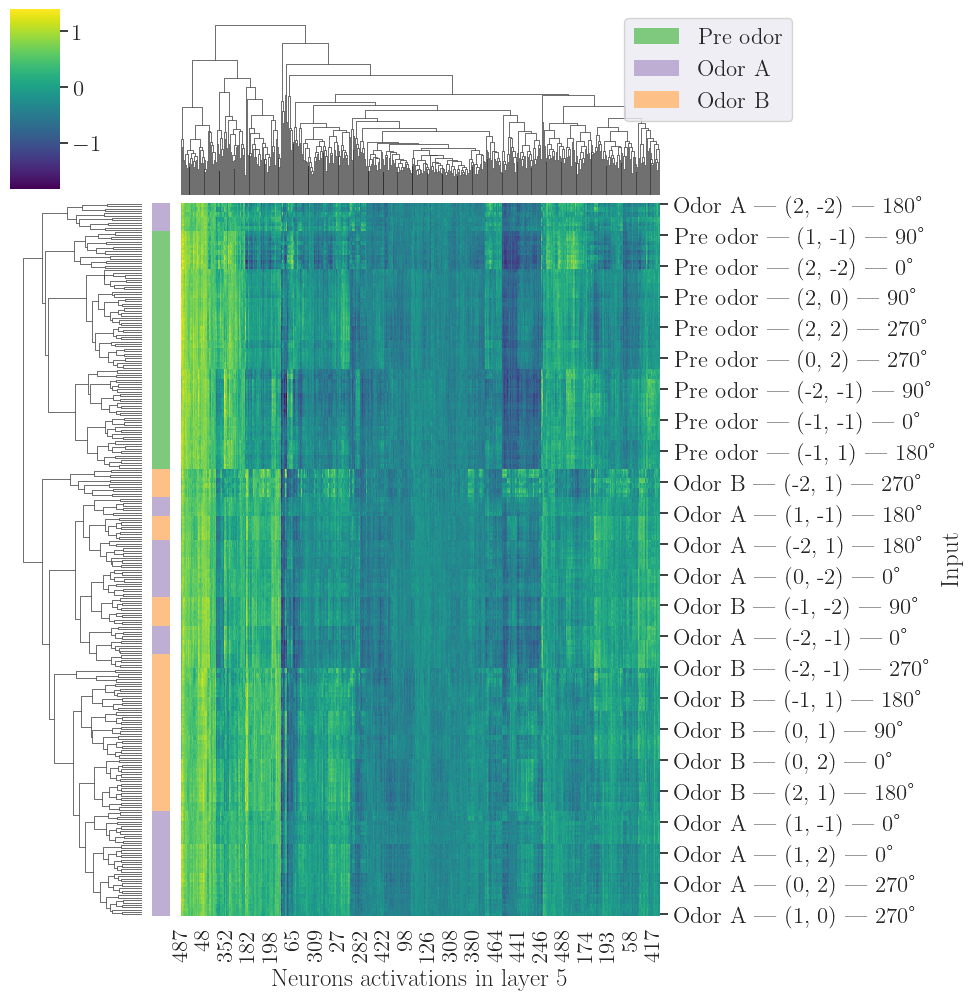
\includegraphics[height=0.9\textheight]{img/activations-learned-EastWest.png}
\end{center}
\end{frame}
\begin{frame}[label={sec:orge4768e5}]{Activations learned - Left/Right}
\begin{center}
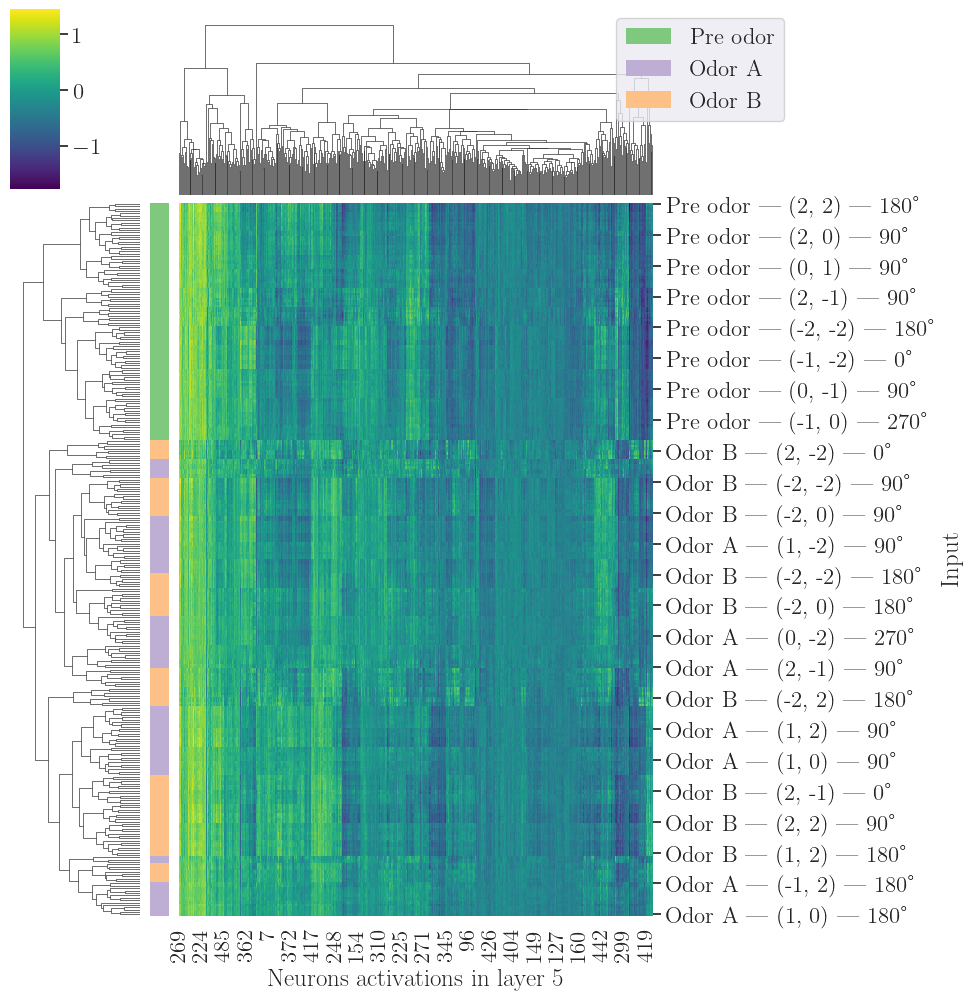
\includegraphics[height=0.9\textheight]{img/activations-learned-LeftRight.png}
\end{center}
\end{frame}
\begin{frame}[label={sec:org83483aa}]{Cluster by action space}
\end{frame}
\begin{frame}[label={sec:org303b966}]{Other clustering method}
\end{frame}
\begin{frame}[<+->][label={sec:org43cf319}]{Use the behavior as proxy -- Perturbation experiment}
\begin{itemize}
\item Perturb the Cartesian/polar part of the input on a trained agent and look at how the agent behaves (x4 experiments)
\item Expectation:
\begin{itemize}
\item Left/right task:
\begin{itemize}
\item With the \alert{Cartesian} inputs perturbed \(\to\) agent's performance unchanged
\item With the \alert{polar} inputs perturbed \(\to\) agent's performance degrades
\end{itemize}
\item East/west task:
\begin{itemize}
\item With the \alert{polar} inputs perturbed \(\to\) agent's performance unchanged
\item With the \alert{Cartesian} inputs perturbed \(\to\) agent's performance degrades
\end{itemize}
\end{itemize}
\end{itemize}
\end{frame}
\begin{frame}[<+->][label={sec:org2ad9d53}]{Use the behavior as proxy -- Perturbation experiment}
\begin{itemize}
\item Cartesian perturbation
\item Polar perturbation
\begin{itemize}
\item Simulation does not end \(\to\) haven't figured out why yet
\end{itemize}
\end{itemize}
\end{frame}
\begin{frame}[label={sec:org993e633}]{Next steps}
\end{frame}
\begin{frame}[label={sec:org0f1a1d7},standout]{~}
Questions ?
\end{frame}
\end{document}
